\chapter{Økonomi}
\section{Indledning}
Eksistensberettigelse for telesundhed – økonomisk besparelse og effektivisering, men er virkeligheden også sådan? Det vil der blive set nærmere på.

Økonomiafsnittet har til formål at belyse omkostningerne ved henholdsvis fysisk hjemmepleje og virtuel hjemmepleje i Favrskov Kommune, og derefter pointere økonomiske forskelle mellem de to scenarier ved hjælp af en ressourceopgørelse.

Følgende spørgsmål ønskes besvaret i økonomiafsnittet:
\begin{itemize}
	\item Hvilke økonomiske konsekvenser medfører implementering af telesundhed?
	\item Er der økonomisk gevinst ved at implementere videoopkald, som erstatning for fysiske besøg i Favrskov Kommune?
\end{itemize}

\section{Metode}
Gennem møder med Appinux, Netplan Care og Favrskov Kommune er det nødvendige udstyr for at kunne implementere telesundhed – herunder virtuel hjemmepleje – blevet identificeret. 
Der er tilegnet informationer om diverse omkostninger ved dette udstyr, samt yderligere omkring arbejdsgange i Favrskov Kommune. 
Priserne til produktet er vejledende og ikke nødvendigvis gældende for Favrskov kommune. Det skyldes, at priserne der er opgivet af Appinux blot er liste priser, og der tages ikke højde for særlige tilbud. 
Yderligere økonomiske konsekvenser er forsøgt klarlagt gennem en søgning af studier omhandlende videobaserede telesundheds løsninger for hjemmepleje på følgende fem databaser: PubMed, Embase, CINAHL, Cochrane Libary og Google Scholar. Google i al almindelighed er ligeledes benyttet til at samle generel information om telesundhed. 

\section{Resultater}
\subsection{Omkostninger ved Telesundhed (Appinux)}
\subsubsection{Opstartsomkostninger}
Opstartsomkostningerne for Appinux’ telesundhedsløsning med skærmopkald ses i nedenstående tabel. Der er vigtigt at pointere, at indkøb af tablets til selve skærmopkaldende ikke er inddraget i opstartsomkostningerne. Det skyldes, at denne udgift er afhængig af typen af tablets der indkøbes, samt antallet af borgere, der skal have en tablet til rådighed. 
Det har hverken været muligt, at få informationer omkring, hvilken type tablet der anbefales fra Appinux, eller antallet af borgere, der potentielt skal benytte telesundhed i Favrskov Kommune.

\begin{figure}[H]
	\centering
	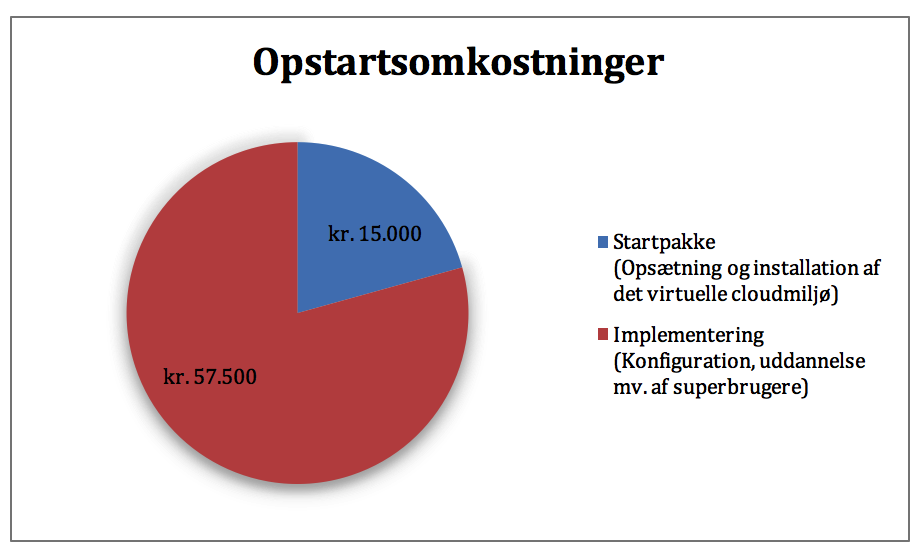
\includegraphics[width=1\textwidth]{Figurer/Snip20160504_26}
	\caption{Opstartsomkostninger for skærmopkald. INDSÆT REFERENCE – MICHAEL ELLEGAARD FRA APPINUX!}
\end{figure}

\subsubsection{Driftsomkostninger}
\textit{Månedligt abonnement}\\
Der tages udgangspunkt i Appinux’ løsning for skærmopkald, hvor der betales et månedligt beløb. Abonnementet varierer i pris alt efter, hvilke moduler der tilkøbes og hvor mange brugere der er. 
Nedenstående tabel skitserer de månedlige udgifter ved skærmopkaldsmodulet ”Platform – Forløb, Kalender, Video”, som er modulet der muliggør videoopkald.

\begin{figure}[H]
	\centering
	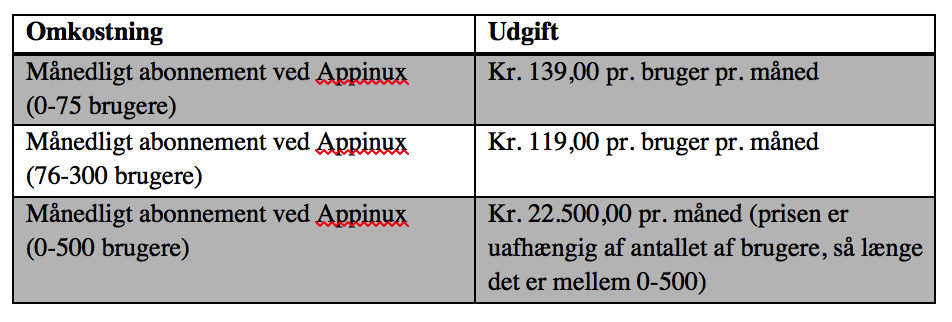
\includegraphics[width=1\textwidth]{Figurer/Snip20160504_27}
	\caption{Tabel over variable driftsomkostninger alt efter antallet af brugere}
\end{figure}

\begin{figure}[H]
	\centering
	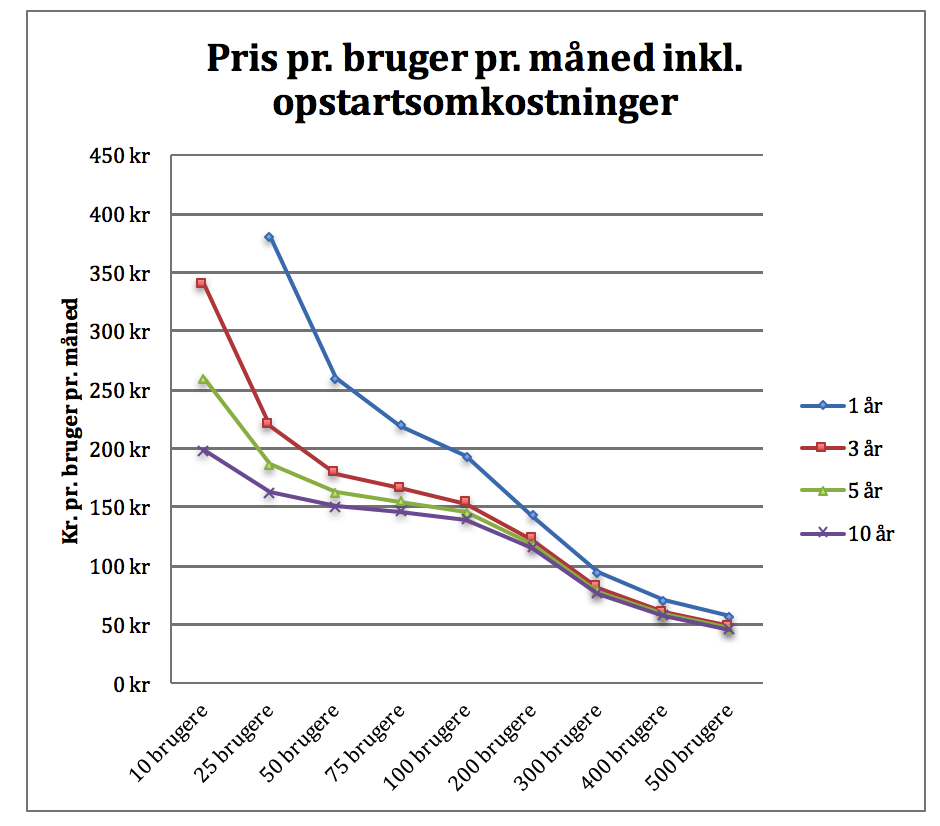
\includegraphics[width=1\textwidth]{Figurer/Snip20160504_28}
	\caption{Pris pr. bruger pr. år inkl. opstartsomkostninger.  Kurven viser den umiddelbare pris for erhvervelse af telesundhedsløsning med videoopkald fra Appinux. Det er ikke et fuldgyldigt billede af prisen for skærmopkald, men blot et billede af, hvordan prisen er afhængig af tid og antal brugere.}
\end{figure}

\textit{Løn til personale}
\begin{itemize}
	\item Support(Fælles servicecenter)
	\item Call center
	\item Opdateringer
\end{itemize}

\textit{Totalomkostninger}

\subsubsection{Omkostninger ved fysiske besøg}
\begin{itemize}
	\item Transportomkostninger INDDRAG ARTIKEL 7 OG 10 - PUBMED
	\item Løn til personale
\end{itemize}

\subsubsection{Ressourceopgørelse}
\begin{itemize}
	\item Appinux vs. fysiske besøg(pris pr. hjulpet borger)
	\item Indirekte økonomiske besparelser ved Telesundhed
	\item Færre indlæggelser, mere selvhjulpne
	\item Mere effektivt – kan hjælpe flere brugere på kortere tid
	\item Bedre udnyttelse af medarbejdernes tid
\end{itemize}

\subsubsection{Usikkerheder}
\begin{itemize}
	\item Yderligere omkostninger
	\item Omfang af målgruppen
	\item Tid brugt på opdatering
	\item Ugennemsigtige priser?
\end{itemize}





\section{Diskussion}
\begin{itemize}
	\item Andre alternativer(fx Viewcare)
	\item Anden type betaling(ikke abonnement) – fordel/ulempe?
	\item Mulighed for udvidelse af ydelser(fx TOBS)? 
	\item Monopol på markedet
	\item Er der økonomisk gevinst ved at implementere Telesundhed i Favrskov Kommune ift. fysiske hjemmebesøg? INDDRAG ARTIKEL 6
	\item Kortsigtet
	\item Langsigtet
	\item Økonomiske udslagsgivende faktorer(fx antal borgere der benytter ydelsen)
	\item Fremtidige økonomiske fordele
	\item Andre ydelser(genoptræning, sårbehandling, psykiatri, mv.)
\end{itemize}
\section{Konklusion}